\begin{frame}[hasprev=false, hasnext=true]
\frametitle{Cause-effect graph example}
\label{example:cause-effect-graph}

\begin{block}{Specification}
The character in column 1 must be an ``A'' or a ``B''. The character is column
2 must be a digit. In this situation, the file must be updated. If the first
character is incorrect, the message X12 must be issued. If the second character
is not a digit, the message X13 must be issued.
\end{block}

\begin{block}{Causes}
\begin{itemize}
	\item \textbf{(1)} Character in column 1 is ``A''.
	\item \textbf{(2)} Character in column 1 is ``B''.
	\item \textbf{(3)} Character in column 2 is a digit.
\end{itemize}
\end{block}

\begin{block}{Effects}
\begin{itemize}
	\item \textbf{(70)} file is updated.
	\item \textbf{(71)} message X12 is issued.
	\item \textbf{(72)} message X13 is issued.
\end{itemize}
\end{block}
\end{frame}



\begin{frame}[hasprev=true, hasnext=true]
\frametitle{Cause-effect graph example}

\begin{block}{Cause-effect graph}
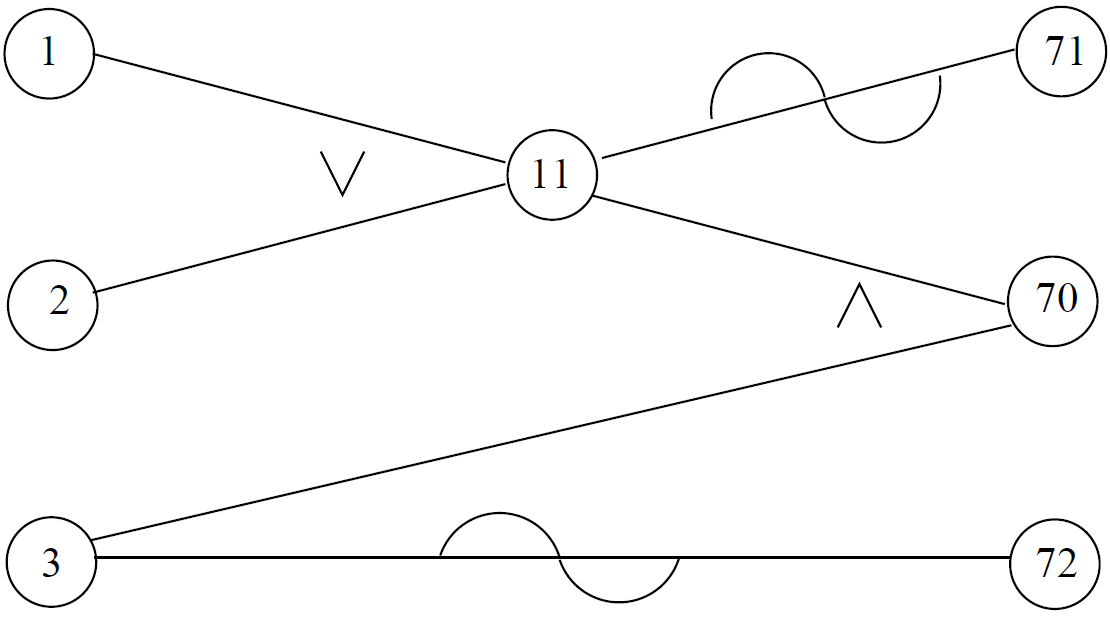
\includegraphics[width=\textwidth]{aux/examples/cause-effect-graph/Cause-effect graph example}
\end{block}

\end{frame}


\begin{frame}
\frametitle{Cause-effect graph example}

\begin{block}{Cause-effect graph (with constraints)}
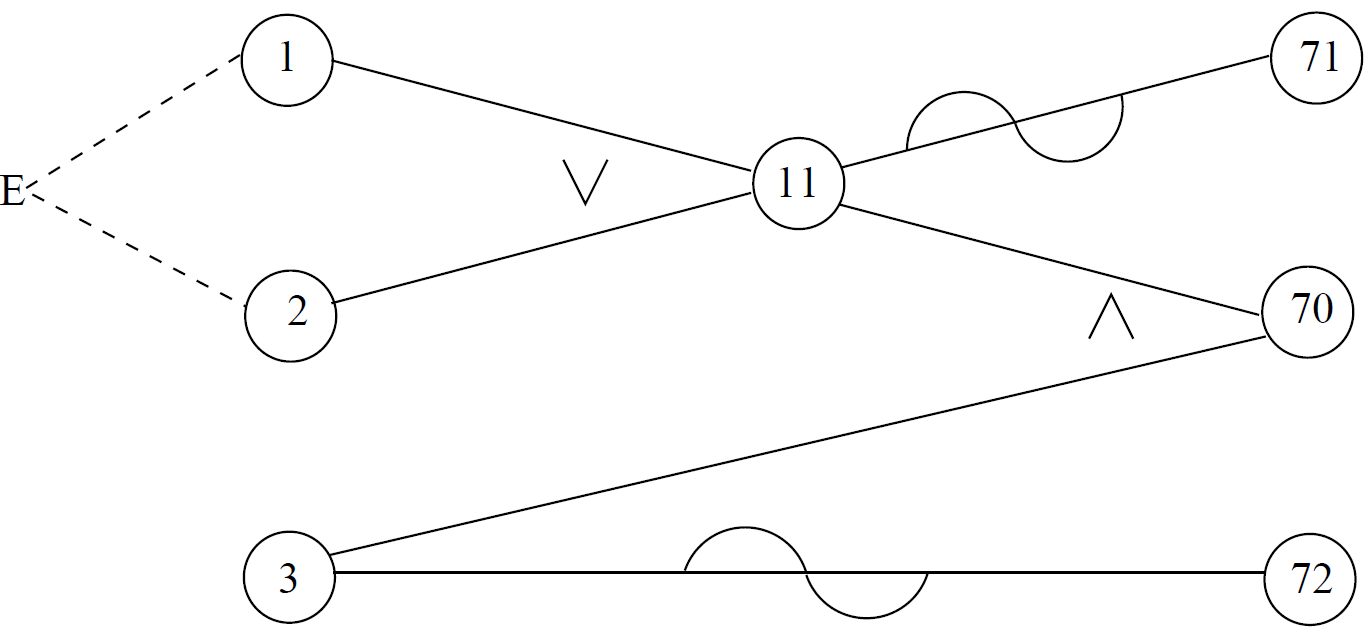
\includegraphics[width=\textwidth]{aux/examples/cause-effect-graph/Cause-effect graph example (with constraints)}
\end{block}
\end{frame}



\begin{frame}[hasprev=true, hasnext=false]
\frametitle{Cause-effect graph example}

\begin{block}{Digital circuit}
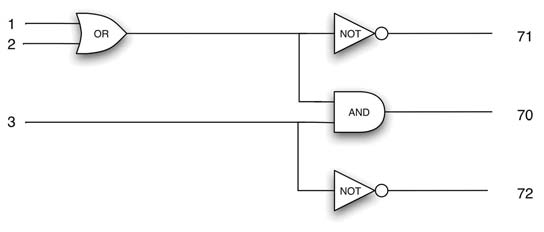
\includegraphics[width=\textwidth]{aux/examples/cause-effect-graph/Cause-effect graph to digital circuit example}
\end{block}

\end{frame}